\documentclass[20pt,margin=1.5in,innermargin=-5.5in,blockverticalspace=-0.25in]{tikzposter}
\geometry{paperwidth=42in,paperheight=30in}
\usepackage[utf8]{inputenc}
\usepackage{amsmath}
\usepackage{amsfonts}
\usepackage{amsthm}
\usepackage{amssymb}
\usepackage{mathrsfs}
\usepackage{graphicx}
\usepackage{adjustbox}
\usepackage{enumitem}
\usepackage[backend=biber,style=numeric]{biblatex}
\usepackage{emory-theme}
\usepackage{hyperref}

\usepackage{mwe} % for placeholder images

\addbibresource{refs.bib}

% set theme parameters
\tikzposterlatexaffectionproofoff
\usetheme{EmoryTheme}
\usecolorstyle{EmoryStyle}

\title{Arccosine Function}
\author{Himansi Maheshkumar Patel ID: 40072262}
\institute{Gina Cody School of Engineering and Computer Science, Concordia University\\}
\titlegraphic{
\includegraphics{Concordia.jpeg}}

% begin document
\begin{document}
\maketitle
\centering
\begin{columns}
    \column{0.33}
    \block{Introduction}{
         The arccosine is the inverse trigonometric function.The arccosine indicates the angle whose cosine is x. The arccosine of x is defined as the inverse cosine function of x when -1 $\leq$ x $\leq$ 1.\\
When the cosine of y is equal to $x: cos y = x$. Then the arccosine of x is equal to the inverse cosine function of x, which is equal to {\centering\textbf{$y: \arccos x = \cos^{-1} x = y$.}}\\
The Taylor's series for arccosine function is :\newline
   \begin{itemize}
        \item The domain of $\arccos x $ is  -1 $\leq$ x $\leq$ 1.
        \item The range of $\arccos x $ is  0 $\leq$ y $\leq$ $\pi$ in radians or $0^{\circ}$$\leq$ y $\leq$$180^{\circ}$ in degrees.
        \item The arccosine function is a reflection of the cosine function about the line $y=x$.
        \item The arccosine function is continuous on open interval (-1,1)
 
    \end{itemize}
       \begin{tikzfigure}[arccosine Function]
        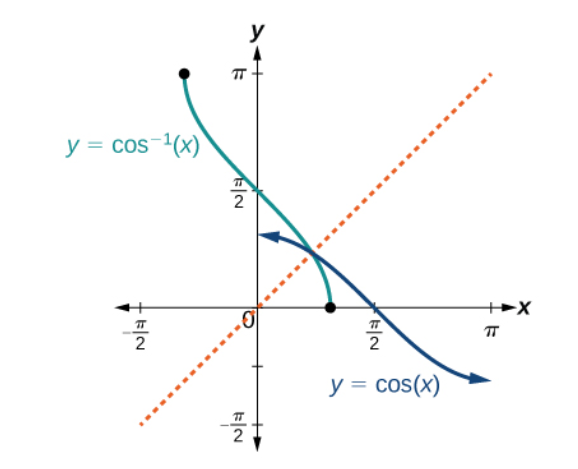
\includegraphics[width=0.9\linewidth]{Capturelast.PNG}
    \end{tikzfigure}
    \begin{itemize}
    \item It is also useful in application of engineering, physics and others.
    \end{itemize}
    }
    \block{Problem 1 - Function Description}{
    \begin{itemize}
        \item Finding precise information about arccosine function especially its unique characteristics was quite hard. I needed to search into various sources and find a source with the right information. 
        \item Learned about arccosine function, its domain \& range, and its applications about which I was not completely aware of!
        \item Learned a new language called ‘LaTeX’ for writing a document in very short time. 
    \end{itemize}
    }
    \column{0.34}
    \block{Problem 2 - Function Requirements}{
    \begin{itemize}
        \item Decided functional and non-functional requirements for arccosine function to see whether some of them would work or not in the future?
        \item After researching on ISO/IEC/IEEE 29148 Standards, I got to know about standard ways by which we can define functional and non-functional requirements in context of software development.
    \end{itemize}
    }
    \block{Problem 3 - Algorithm}{
    \begin{itemize}
        \item Brainstormed with my team to decide an identical pseudocode format which can be useful for team members when reviewing code.
        \item After exploring various possible approaches to solve arccosine function, using Taylor's series for its evaluation seemed most appropriate.
        \begin{align*} 
        \arccos x = \frac{\pi}{2}-\sum_{n=0}^\infty\frac{(2n)!}{2^{2n}(n!)^{2}}\frac{x^{2n+1}}{(2n+1)},|x|\textless1\\ 
        \end{align*}
        \item In order to arrive at an optimal solution, from a performance perspective, I tried implementing and further comparing an iterative version of the algorithm against a recursive one and decided to use iterative approach.
        \item Learned about implementing an algorithm using a Taylor series.
    \end{itemize}
    }
    \block{Problem 4 - Implementation}{
    \begin{itemize}
        \item Brainstormed with my team to choose a common programming style which makes it easier to review codes for others.
        \item Generally, it seems more logical to go for a GUI when the system offers a variety of options to an End-User for interacting with the application. Considering our application requirements which primarily involved limited user interaction only in form of taking user inputs I found using a textual interface better than a complex GUI.
        \item Learned about implementing the arccosine function from a scratch since I didn’t have access to any in-built library.
        \item While implementing arccosine function, I learned about error handling mechanism and how useful an error message can be for the users.
        \item Learned about ways to implement a program which makes it correct, efficient, usable and robust.
        \item I had never used checkstyle before. I came to know the use of checkstyle in project.
        \item Learned about agile principles.
    \end{itemize}
    }
    \column{0.33}
    \block{Problem 5 - Code Review}{
    \begin{itemize}
        \item When I implemented a program, I didn’t know that I could use static method for the utility function. But, after getting review from teammate, I came to know about static method. I then searched on internet that in which context I can make method static. Then I realized that I could have used static method for my function as well. 
        \item Got to know the importance of working in a team that how reviewing team member’s code can be useful in sharing knowledge, finding early bugs, team cohesion and maintaining consistent code style in a group.
        \item Learned about manual and automatic code review approach. 
        \item Used \textbf{PMD} tool to check the quality of source code which was a new lesson for me.
    \end{itemize}
    }
    
    \block{Problem 6 - Testing}{
    \begin{itemize}
        \item Decided to make testcase methods based on arccosine function’s requirements as it finds early bugs, reduces the cost of bug fixes, and stops program from failing. For implementing this, I used standard unit testing framework known as ‘Junit”.
        \item Arccosine function was not able to provide accurate result up to 4 decimal points for some domain values so I had to make a decision to check arccosine function’s results up to 2 decimal points only.
        \item Learned how to write testcase methods which can cover all possible the testcases.
    \end{itemize}
    }
    \block{Problem 7 - Test Case Analysis}{
    \begin{itemize}
        \item From testcase analysis approach, I came to know about different steps of functional testing, how to perform it, and how to report it.
        \item Learned about importance of test case analysis report to the developer as it helps them in finding out failing testcases.
    \end{itemize}
    }
    
    \block{GitHub Link}{
            https://github.com/Himansipatel/SOEN-6011-Team-H-Himansi
    }
\end{columns}
\end{document}